\documentclass[a4paper]{book}
\usepackage{makeidx}
\usepackage{natbib}
\usepackage{graphicx}
\usepackage{multicol}
\usepackage{float}
\usepackage{listings}
\usepackage{color}
\usepackage{ifthen}
\usepackage[table]{xcolor}
\usepackage{textcomp}
\usepackage{alltt}
\usepackage{ifpdf}
\ifpdf
\usepackage[pdftex,
            pagebackref=true,
            colorlinks=true,
            linkcolor=blue,
            unicode
           ]{hyperref}
\else
\usepackage[ps2pdf,
            pagebackref=true,
            colorlinks=true,
            linkcolor=blue,
            unicode
           ]{hyperref}
\usepackage{pspicture}
\fi
\usepackage[utf8]{inputenc}
\usepackage{mathptmx}
\usepackage[scaled=.90]{helvet}
\usepackage{courier}
\usepackage{sectsty}
\usepackage[titles]{tocloft}
\usepackage{doxygen}
\lstset{language=C++,inputencoding=utf8,basicstyle=\footnotesize,breaklines=true,breakatwhitespace=true,tabsize=8,numbers=left }
\makeindex
\setcounter{tocdepth}{3}
\renewcommand{\footrulewidth}{0.4pt}
\renewcommand{\familydefault}{\sfdefault}
\hfuzz=15pt
\setlength{\emergencystretch}{15pt}
\hbadness=750
\tolerance=750
\begin{document}
\hypersetup{pageanchor=false,citecolor=blue}
\begin{titlepage}
\vspace*{7cm}
\begin{center}
{\Large \-Net\-Sim }\\
\vspace*{1cm}
{\large \-Generated by Doxygen 1.7.6.1}\\
\vspace*{0.5cm}
{\small Tue Dec 10 2013 16:35:24}\\
\end{center}
\end{titlepage}
\clearemptydoublepage
\pagenumbering{roman}
\tableofcontents
\clearemptydoublepage
\pagenumbering{arabic}
\hypersetup{pageanchor=true,citecolor=blue}
\chapter{\-Network \-Simulator \-Documentation}
\label{index}\hypertarget{index}{}\input{index}
\chapter{\-Class \-Index}
\section{\-Class \-Hierarchy}
\-This inheritance list is sorted roughly, but not completely, alphabetically\-:\begin{DoxyCompactList}
\item \contentsline{section}{\-Congestion\-Alg}{\pageref{classCongestionAlg}}{}
\item \contentsline{section}{\-Event}{\pageref{classEvent}}{}
\begin{DoxyCompactList}
\item \contentsline{section}{\-Flow\-Event}{\pageref{classFlowEvent}}{}
\item \contentsline{section}{\-Packet\-Event}{\pageref{classPacketEvent}}{}
\item \contentsline{section}{\-Unack\-Event}{\pageref{classUnackEvent}}{}
\end{DoxyCompactList}
\item \contentsline{section}{\-Event\-Generator}{\pageref{classEventGenerator}}{}
\begin{DoxyCompactList}
\item \contentsline{section}{\-Flow\-Generator}{\pageref{classFlowGenerator}}{}
\item \contentsline{section}{\-Host}{\pageref{classHost}}{}
\item \contentsline{section}{\-Link}{\pageref{classLink}}{}
\item \contentsline{section}{\-Router}{\pageref{classRouter}}{}
\end{DoxyCompactList}
\item \contentsline{section}{\-Flow}{\pageref{classFlow}}{}
\item \contentsline{section}{\-Handler}{\pageref{classHandler}}{}
\item \contentsline{section}{\-Log$<$ \-T $>$}{\pageref{classLog}}{}
\item \contentsline{section}{\-Log$<$ \-Output2\-F\-I\-L\-E $>$}{\pageref{classLog}}{}
\begin{DoxyCompactList}
\item \contentsline{section}{\-F\-I\-L\-E\-Log}{\pageref{classFILELog}}{}
\end{DoxyCompactList}
\item \contentsline{section}{\-Output2\-F\-I\-L\-E}{\pageref{classOutput2FILE}}{}
\item \contentsline{section}{\-Packet}{\pageref{classPacket}}{}
\end{DoxyCompactList}

\chapter{\-Class \-Index}
\section{\-Class \-List}
\-Here are the classes, structs, unions and interfaces with brief descriptions\-:\begin{DoxyCompactList}
\item\contentsline{section}{\hyperlink{classBFResendEvent}{\-B\-F\-Resend\-Event} \\*\-A \hyperlink{classBFResendEvent}{\-B\-F\-Resend\-Event} will be used to \-Routers to resend their information for \-Bellman-\/\-Ford }{\pageref{classBFResendEvent}}{}
\item\contentsline{section}{\hyperlink{classEvent}{\-Event} \\*\-Abstract class representing a generic \hyperlink{classEvent}{\-Event} in our \hyperlink{classEvent}{\-Event} based simulation }{\pageref{classEvent}}{}
\item\contentsline{section}{\hyperlink{classEventGenerator}{\-Event\-Generator} \\*\-Superclass for \-Links, \-Hosts, \-Routers, and \-Flow\-Generators }{\pageref{classEventGenerator}}{}
\item\contentsline{section}{\hyperlink{classFlow}{\-Flow} }{\pageref{classFlow}}{}
\item\contentsline{section}{\hyperlink{classFlowEvent}{\-Flow\-Event} }{\pageref{classFlowEvent}}{}
\item\contentsline{section}{\hyperlink{classFlowGenerator}{\-Flow\-Generator} \\*\-An object used to store \hyperlink{classFlow}{\-Flow} objects until the data flow is ready to begin }{\pageref{classFlowGenerator}}{}
\item\contentsline{section}{\hyperlink{classHandler}{\-Handler} \\*\hyperlink{classHandler}{\-Handler} that runs the \-Event-\/based simulation }{\pageref{classHandler}}{}
\item\contentsline{section}{\hyperlink{classHost}{\-Host} }{\pageref{classHost}}{}
\item\contentsline{section}{\hyperlink{classLink}{\-Link} }{\pageref{classLink}}{}
\item\contentsline{section}{\hyperlink{classPacket}{\-Packet} \\*\-A class to represent \-Packets in the network }{\pageref{classPacket}}{}
\item\contentsline{section}{\hyperlink{classPacketEvent}{\-Packet\-Event} \\*\-A wrapper for the \hyperlink{classPacket}{\-Packet} class }{\pageref{classPacketEvent}}{}
\item\contentsline{section}{\hyperlink{classPath}{\-Path} }{\pageref{classPath}}{}
\item\contentsline{section}{\hyperlink{classRouter}{\-Router} }{\pageref{classRouter}}{}
\item\contentsline{section}{\hyperlink{classTahoeFlow}{\-Tahoe\-Flow} }{\pageref{classTahoeFlow}}{}
\item\contentsline{section}{\hyperlink{classTCPVegasUpdateEvent}{\-T\-C\-P\-Vegas\-Update\-Event} \\*\-A mechanism by which \hyperlink{classVegasFlow}{\-Vegas\-Flow} algorithms are called to update their window sizes }{\pageref{classTCPVegasUpdateEvent}}{}
\item\contentsline{section}{\hyperlink{classUnackEvent}{\-Unack\-Event} \\*\-An \hyperlink{classUnackEvent}{\-Unack\-Event} is called when an \hyperlink{classEvent}{\-Event} times out }{\pageref{classUnackEvent}}{}
\item\contentsline{section}{\hyperlink{classVegasFlow}{\-Vegas\-Flow} }{\pageref{classVegasFlow}}{}
\end{DoxyCompactList}

\chapter{\-Class \-Documentation}
\input{classBFResendEvent}
\hypertarget{classEvent}{\section{\-Event \-Class \-Reference}
\label{classEvent}\index{\-Event@{\-Event}}
}


\-Abstract class representing a generic \hyperlink{classEvent}{\-Event} in our \hyperlink{classEvent}{\-Event} based simulation.  




{\ttfamily \#include $<$\-Event.\-h$>$}

\-Inheritance diagram for \-Event\-:\begin{figure}[H]
\begin{center}
\leavevmode
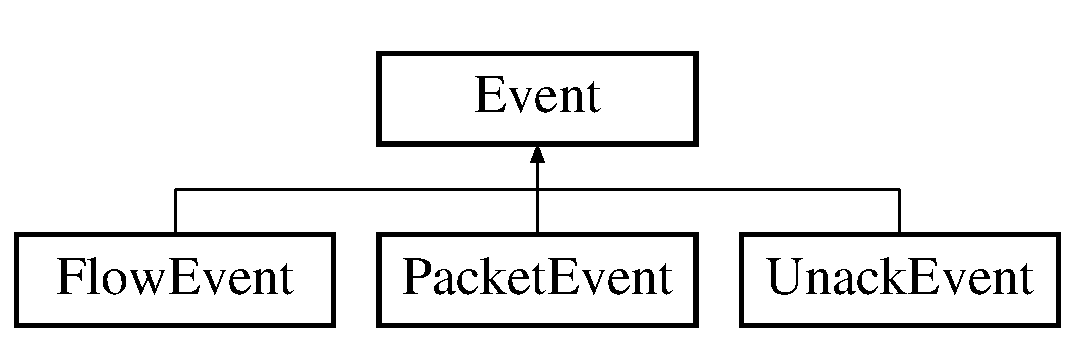
\includegraphics[height=1.483444cm]{classEvent}
\end{center}
\end{figure}
\subsection*{\-Public \-Member \-Functions}
\begin{DoxyCompactItemize}
\item 
\hyperlink{classEvent_a2ff6ddc14b006baade2b5ab2a622835d}{\-Event} (std\-::string dest, std\-::string src, double ts)
\begin{DoxyCompactList}\small\item\em \-Constructor for a generic \hyperlink{classEvent}{\-Event}. \end{DoxyCompactList}\item 
\hypertarget{classEvent_a79ba42604867e6f81ec29d9eaff0dc08}{double \hyperlink{classEvent_a79ba42604867e6f81ec29d9eaff0dc08}{event\-Time} () const }\label{classEvent_a79ba42604867e6f81ec29d9eaff0dc08}

\begin{DoxyCompactList}\small\item\em \-Get the time of the \hyperlink{classEvent}{\-Event}. \end{DoxyCompactList}\item 
\hypertarget{classEvent_a924194a887aa70888e08a04b69389bd6}{virtual std\-::string \hyperlink{classEvent_a924194a887aa70888e08a04b69389bd6}{to\-String} ()}\label{classEvent_a924194a887aa70888e08a04b69389bd6}

\begin{DoxyCompactList}\small\item\em \-Get a string representing the \hyperlink{classEvent}{\-Event}. \end{DoxyCompactList}\item 
\hypertarget{classEvent_a3e3dfee48cea1b42321adae3c51f82e2}{virtual std\-::string \hyperlink{classEvent_a3e3dfee48cea1b42321adae3c51f82e2}{get\-Type} ()}\label{classEvent_a3e3dfee48cea1b42321adae3c51f82e2}

\begin{DoxyCompactList}\small\item\em \-Get the type of the \hyperlink{classEvent}{\-Event}, as a string. \end{DoxyCompactList}\end{DoxyCompactItemize}
\subsection*{\-Public \-Attributes}
\begin{DoxyCompactItemize}
\item 
std\-::string \hyperlink{classEvent_aa28be1a89b2516ea9f570ff619f754bc}{destination}
\begin{DoxyCompactList}\small\item\em \-The destination of the \hyperlink{classEvent}{\-Event}. \end{DoxyCompactList}\item 
std\-::string \hyperlink{classEvent_abc9c246c173d3433d2ffc0a4ed35bc01}{source}
\begin{DoxyCompactList}\small\item\em \-The source of the \hyperlink{classEvent}{\-Event}. \end{DoxyCompactList}\end{DoxyCompactItemize}
\subsection*{\-Protected \-Attributes}
\begin{DoxyCompactItemize}
\item 
\hypertarget{classEvent_abf947fd0c5db2bf468373ee94ec190b4}{double {\bfseries timestamp}}\label{classEvent_abf947fd0c5db2bf468373ee94ec190b4}

\end{DoxyCompactItemize}


\subsection{\-Detailed \-Description}
\-Abstract class representing a generic \hyperlink{classEvent}{\-Event} in our \hyperlink{classEvent}{\-Event} based simulation. 

\subsection{\-Constructor \& \-Destructor \-Documentation}
\hypertarget{classEvent_a2ff6ddc14b006baade2b5ab2a622835d}{\index{\-Event@{\-Event}!\-Event@{\-Event}}
\index{\-Event@{\-Event}!Event@{\-Event}}
\subsubsection[{\-Event}]{\setlength{\rightskip}{0pt plus 5cm}{\bf \-Event\-::\-Event} (
\begin{DoxyParamCaption}
\item[{std\-::string}]{dest, }
\item[{std\-::string}]{src, }
\item[{double}]{ts}
\end{DoxyParamCaption}
)}}\label{classEvent_a2ff6ddc14b006baade2b5ab2a622835d}


\-Constructor for a generic \hyperlink{classEvent}{\-Event}. 


\begin{DoxyParams}{\-Parameters}
{\em dest} & the destination of the \hyperlink{classEvent}{\-Event} (where the \hyperlink{classEvent}{\-Event} should land). \\
\hline
{\em src} & the creator of the \hyperlink{classEvent}{\-Event}. \\
\hline
{\em ts} & the time at which the event is fired \\
\hline
\end{DoxyParams}


\subsection{\-Member \-Data \-Documentation}
\hypertarget{classEvent_aa28be1a89b2516ea9f570ff619f754bc}{\index{\-Event@{\-Event}!destination@{destination}}
\index{destination@{destination}!Event@{\-Event}}
\subsubsection[{destination}]{\setlength{\rightskip}{0pt plus 5cm}std\-::string {\bf \-Event\-::destination}}}\label{classEvent_aa28be1a89b2516ea9f570ff619f754bc}


\-The destination of the \hyperlink{classEvent}{\-Event}. 

\hypertarget{classEvent_abc9c246c173d3433d2ffc0a4ed35bc01}{\index{\-Event@{\-Event}!source@{source}}
\index{source@{source}!Event@{\-Event}}
\subsubsection[{source}]{\setlength{\rightskip}{0pt plus 5cm}std\-::string {\bf \-Event\-::source}}}\label{classEvent_abc9c246c173d3433d2ffc0a4ed35bc01}


\-The source of the \hyperlink{classEvent}{\-Event}. 



\-The documentation for this class was generated from the following files\-:\begin{DoxyCompactItemize}
\item 
/home/max/caltech/\-Net\-Sim/\-C\-S\-\_\-143/src/\-Event\-Handling/\-Event.\-h\item 
/home/max/caltech/\-Net\-Sim/\-C\-S\-\_\-143/src/\-Event\-Handling/\-Event.\-cpp\end{DoxyCompactItemize}

\hypertarget{classEventGenerator}{\section{\-Event\-Generator \-Class \-Reference}
\label{classEventGenerator}\index{\-Event\-Generator@{\-Event\-Generator}}
}


\-Superclass for \-Links, \-Hosts, \-Routers, and \-Flow\-Generators.  




{\ttfamily \#include $<$\-Event\-Generator.\-h$>$}

\-Inheritance diagram for \-Event\-Generator\-:\begin{figure}[H]
\begin{center}
\leavevmode
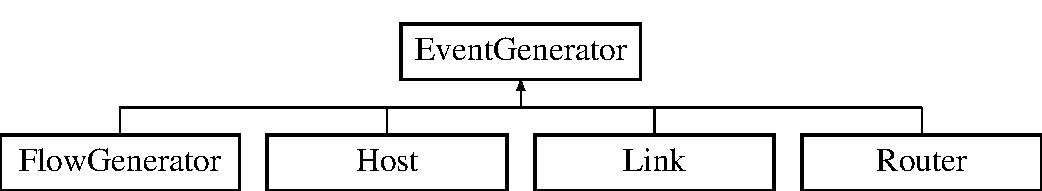
\includegraphics[height=2.000000cm]{classEventGenerator}
\end{center}
\end{figure}
\subsection*{\-Public \-Member \-Functions}
\begin{DoxyCompactItemize}
\item 
std\-::string \hyperlink{classEventGenerator_a467b319c4317b83b9c16708c9815953d}{get\-I\-D} () const 
\begin{DoxyCompactList}\small\item\em \-Get the \-I\-D of the \hyperlink{classEventGenerator}{\-Event\-Generator}. \end{DoxyCompactList}\item 
virtual void \hyperlink{classEventGenerator_a7448c87e533a9b38c20d914fa6a13c8e}{give\-Event} (std\-::shared\-\_\-ptr$<$ \hyperlink{classEvent}{\-Event} $>$ e)=0
\begin{DoxyCompactList}\small\item\em \-Hands an \hyperlink{classEvent}{\-Event} to the \hyperlink{classEventGenerator}{\-Event\-Generator} for processing. \end{DoxyCompactList}\item 
bool \hyperlink{classEventGenerator_a1fd7fdcaa263115e89a9fc69b85eca22}{has\-Events} ()
\begin{DoxyCompactList}\small\item\em \-Tells whether the \hyperlink{classEventGenerator}{\-Event\-Generator}'s priority queue has any events. \end{DoxyCompactList}\item 
std\-::shared\-\_\-ptr$<$ \hyperlink{classEvent}{\-Event} $>$ \hyperlink{classEventGenerator_ab40fd3a0bf1aa974ba50feb443d81009}{get\-Event} ()
\begin{DoxyCompactList}\small\item\em \-Remove and return the lowest time event from the \hyperlink{classEventGenerator}{\-Event\-Generator}'s priority queue. \end{DoxyCompactList}\item 
double \hyperlink{classEventGenerator_ac4b5ccdeaf232fe59854535bb13747a9}{get\-Next\-Time} ()
\begin{DoxyCompactList}\small\item\em \-Get the lowest time in the \hyperlink{classEventGenerator}{\-Event\-Generator}'s priority queue. \end{DoxyCompactList}\item 
void \hyperlink{classEventGenerator_a3487849484c9b521527d6acacee79e88}{add\-Event\-To\-Local\-Queue} (std\-::shared\-\_\-ptr$<$ \hyperlink{classEvent}{\-Event} $>$ e)
\begin{DoxyCompactList}\small\item\em \-Add \hyperlink{classEvent}{\-Event} to local event\-Heap. \end{DoxyCompactList}\end{DoxyCompactItemize}
\subsection*{\-Public \-Attributes}
\begin{DoxyCompactItemize}
\item 
std\-::string \hyperlink{classEventGenerator_af4fa28d08ed4a3be31f9383cf72e0d2c}{uuid}
\begin{DoxyCompactList}\small\item\em \-The unique id of the \hyperlink{classEventGenerator}{\-Event\-Generator}. \end{DoxyCompactList}\item 
\hypertarget{classEventGenerator_a3e9a33f75d9861bece6c30b5249c9d39}{std\-::priority\-\_\-queue\*
$<$ std\-::shared\-\_\-ptr$<$ \hyperlink{classEvent}{\-Event} $>$\*
, std\-::vector$<$ std\-::shared\-\_\-ptr\*
$<$ \hyperlink{classEvent}{\-Event} $>$ $>$, std\-::greater\*
$<$ std\-::shared\-\_\-ptr$<$ \hyperlink{classEvent}{\-Event} $>$ $>$ $>$ \hyperlink{classEventGenerator_a3e9a33f75d9861bece6c30b5249c9d39}{event\-Heap}}\label{classEventGenerator_a3e9a33f75d9861bece6c30b5249c9d39}

\begin{DoxyCompactList}\small\item\em \-The event\-Heap, which stores a list of events that the the \hyperlink{classEventGenerator}{\-Event\-Generator} will give to the \-Event\-Handler. \end{DoxyCompactList}\end{DoxyCompactItemize}


\subsection{\-Detailed \-Description}
\-Superclass for \-Links, \-Hosts, \-Routers, and \-Flow\-Generators. 

\-Event\-Generators each have their own event\-Heaps, which are ordered lists of events. \-The \-Event\-Handler will determine the \hyperlink{classEvent}{\-Event} in the event\-Heaps of the set of \-Event\-Generators with the minimum time, and handle the \hyperlink{classEvent}{\-Event}. 

\subsection{\-Member \-Function \-Documentation}
\hypertarget{classEventGenerator_a3487849484c9b521527d6acacee79e88}{\index{\-Event\-Generator@{\-Event\-Generator}!add\-Event\-To\-Local\-Queue@{add\-Event\-To\-Local\-Queue}}
\index{add\-Event\-To\-Local\-Queue@{add\-Event\-To\-Local\-Queue}!EventGenerator@{\-Event\-Generator}}
\subsubsection[{add\-Event\-To\-Local\-Queue}]{\setlength{\rightskip}{0pt plus 5cm}void {\bf \-Event\-Generator\-::add\-Event\-To\-Local\-Queue} (
\begin{DoxyParamCaption}
\item[{std\-::shared\-\_\-ptr$<$ {\bf \-Event} $>$}]{e}
\end{DoxyParamCaption}
)}}\label{classEventGenerator_a3487849484c9b521527d6acacee79e88}


\-Add \hyperlink{classEvent}{\-Event} to local event\-Heap. 


\begin{DoxyParams}{\-Parameters}
{\em \-E} & the \hyperlink{classEvent}{\-Event} to add \\
\hline
\end{DoxyParams}
\hypertarget{classEventGenerator_ab40fd3a0bf1aa974ba50feb443d81009}{\index{\-Event\-Generator@{\-Event\-Generator}!get\-Event@{get\-Event}}
\index{get\-Event@{get\-Event}!EventGenerator@{\-Event\-Generator}}
\subsubsection[{get\-Event}]{\setlength{\rightskip}{0pt plus 5cm}std\-::shared\-\_\-ptr$<$ {\bf \-Event} $>$ {\bf \-Event\-Generator\-::get\-Event} (
\begin{DoxyParamCaption}
{}
\end{DoxyParamCaption}
)}}\label{classEventGenerator_ab40fd3a0bf1aa974ba50feb443d81009}


\-Remove and return the lowest time event from the \hyperlink{classEventGenerator}{\-Event\-Generator}'s priority queue. 

\begin{DoxyReturn}{\-Returns}
a pointer to the removed \hyperlink{classEvent}{\-Event}. 
\end{DoxyReturn}
\hypertarget{classEventGenerator_a467b319c4317b83b9c16708c9815953d}{\index{\-Event\-Generator@{\-Event\-Generator}!get\-I\-D@{get\-I\-D}}
\index{get\-I\-D@{get\-I\-D}!EventGenerator@{\-Event\-Generator}}
\subsubsection[{get\-I\-D}]{\setlength{\rightskip}{0pt plus 5cm}std\-::string {\bf \-Event\-Generator\-::get\-I\-D} (
\begin{DoxyParamCaption}
{}
\end{DoxyParamCaption}
) const}}\label{classEventGenerator_a467b319c4317b83b9c16708c9815953d}


\-Get the \-I\-D of the \hyperlink{classEventGenerator}{\-Event\-Generator}. 

\begin{DoxyReturn}{\-Returns}
the \-I\-D as a string 
\end{DoxyReturn}
\hypertarget{classEventGenerator_ac4b5ccdeaf232fe59854535bb13747a9}{\index{\-Event\-Generator@{\-Event\-Generator}!get\-Next\-Time@{get\-Next\-Time}}
\index{get\-Next\-Time@{get\-Next\-Time}!EventGenerator@{\-Event\-Generator}}
\subsubsection[{get\-Next\-Time}]{\setlength{\rightskip}{0pt plus 5cm}double {\bf \-Event\-Generator\-::get\-Next\-Time} (
\begin{DoxyParamCaption}
{}
\end{DoxyParamCaption}
)}}\label{classEventGenerator_ac4b5ccdeaf232fe59854535bb13747a9}


\-Get the lowest time in the \hyperlink{classEventGenerator}{\-Event\-Generator}'s priority queue. 

\begin{DoxyReturn}{\-Returns}
the min time as a double 
\end{DoxyReturn}
\hypertarget{classEventGenerator_a7448c87e533a9b38c20d914fa6a13c8e}{\index{\-Event\-Generator@{\-Event\-Generator}!give\-Event@{give\-Event}}
\index{give\-Event@{give\-Event}!EventGenerator@{\-Event\-Generator}}
\subsubsection[{give\-Event}]{\setlength{\rightskip}{0pt plus 5cm}virtual void {\bf \-Event\-Generator\-::give\-Event} (
\begin{DoxyParamCaption}
\item[{std\-::shared\-\_\-ptr$<$ {\bf \-Event} $>$}]{e}
\end{DoxyParamCaption}
)\hspace{0.3cm}{\ttfamily  \mbox{[}pure virtual\mbox{]}}}}\label{classEventGenerator_a7448c87e533a9b38c20d914fa6a13c8e}


\-Hands an \hyperlink{classEvent}{\-Event} to the \hyperlink{classEventGenerator}{\-Event\-Generator} for processing. 


\begin{DoxyParams}{\-Parameters}
{\em e} & the \hyperlink{classEvent}{\-Event} to be processed. \\
\hline
\end{DoxyParams}


\-Implemented in \hyperlink{classHost_a658a8bee30dfb9e6ff7abc26620f88ff}{\-Host}, \hyperlink{classRouter_aed4bdd88f4fa09cb784c5c329c935688}{\-Router}, \hyperlink{classLink_abd9466c4c2097329f4affd9b2eafbd7a}{\-Link}, and \hyperlink{classFlowGenerator_a9fd8f79663c4af4ab229dde250bc258c}{\-Flow\-Generator}.

\hypertarget{classEventGenerator_a1fd7fdcaa263115e89a9fc69b85eca22}{\index{\-Event\-Generator@{\-Event\-Generator}!has\-Events@{has\-Events}}
\index{has\-Events@{has\-Events}!EventGenerator@{\-Event\-Generator}}
\subsubsection[{has\-Events}]{\setlength{\rightskip}{0pt plus 5cm}bool {\bf \-Event\-Generator\-::has\-Events} (
\begin{DoxyParamCaption}
{}
\end{DoxyParamCaption}
)}}\label{classEventGenerator_a1fd7fdcaa263115e89a9fc69b85eca22}


\-Tells whether the \hyperlink{classEventGenerator}{\-Event\-Generator}'s priority queue has any events. 

\begin{DoxyReturn}{\-Returns}
bool is true if there are events 
\end{DoxyReturn}


\subsection{\-Member \-Data \-Documentation}
\hypertarget{classEventGenerator_af4fa28d08ed4a3be31f9383cf72e0d2c}{\index{\-Event\-Generator@{\-Event\-Generator}!uuid@{uuid}}
\index{uuid@{uuid}!EventGenerator@{\-Event\-Generator}}
\subsubsection[{uuid}]{\setlength{\rightskip}{0pt plus 5cm}std\-::string {\bf \-Event\-Generator\-::uuid}}}\label{classEventGenerator_af4fa28d08ed4a3be31f9383cf72e0d2c}


\-The unique id of the \hyperlink{classEventGenerator}{\-Event\-Generator}. 



\-The documentation for this class was generated from the following files\-:\begin{DoxyCompactItemize}
\item 
/home/max/caltech/\-Net\-Sim/\-C\-S\-\_\-143/src/\-Event\-Generators/\-Event\-Generator.\-h\item 
/home/max/caltech/\-Net\-Sim/\-C\-S\-\_\-143/src/\-Event\-Generators/\-Event\-Generator.\-cpp\end{DoxyCompactItemize}

\hypertarget{classFlow}{\section{\-Flow \-Class \-Reference}
\label{classFlow}\index{\-Flow@{\-Flow}}
}
\subsection*{\-Public \-Member \-Functions}
\begin{DoxyCompactItemize}
\item 
\hypertarget{classFlow_aeb609967880d902a1f8ff8ad9db85862}{{\bfseries \-Flow} (std\-::string idval, std\-::string src, std\-::string dest, std\-::shared\-\_\-ptr$<$ \hyperlink{classCongestionAlg}{\-Congestion\-Alg} $>$ alg, int data\-\_\-size, std\-::shared\-\_\-ptr$<$ \hyperlink{classHost}{\-Host} $>$ h, int win\-Size, float ts)}\label{classFlow_aeb609967880d902a1f8ff8ad9db85862}

\item 
\hypertarget{classFlow_ad7f274b803ded1f3c5b1a4e24e477561}{void {\bfseries handle\-Unack\-Event} (std\-::shared\-\_\-ptr$<$ \hyperlink{classPacket}{\-Packet} $>$ unacked, float time)}\label{classFlow_ad7f274b803ded1f3c5b1a4e24e477561}

\item 
\hypertarget{classFlow_abb3e75cba1b777a083cfa5bae24c7af0}{void {\bfseries handle\-Ack} (std\-::shared\-\_\-ptr$<$ \hyperlink{classPacket}{\-Packet} $>$ p, float time)}\label{classFlow_abb3e75cba1b777a083cfa5bae24c7af0}

\item 
\hypertarget{classFlow_ae330545a178e3800aadb7c3f856b7b94}{std\-::string {\bfseries to\-String} ()}\label{classFlow_ae330545a178e3800aadb7c3f856b7b94}

\item 
\hypertarget{classFlow_a2fdad818f50e010c5db255abfc5138df}{void {\bfseries initialize} ()}\label{classFlow_a2fdad818f50e010c5db255abfc5138df}

\end{DoxyCompactItemize}
\subsection*{\-Public \-Attributes}
\begin{DoxyCompactItemize}
\item 
\hypertarget{classFlow_af45cdc7b3609577eb08cb072e9631809}{std\-::shared\-\_\-ptr$<$ \hyperlink{classHost}{\-Host} $>$ {\bfseries host}}\label{classFlow_af45cdc7b3609577eb08cb072e9631809}

\item 
\hypertarget{classFlow_a8724a8f4ce94cf7bfb0db79e688ed179}{std\-::string {\bfseries id}}\label{classFlow_a8724a8f4ce94cf7bfb0db79e688ed179}

\item 
\hypertarget{classFlow_a36eb3e23b0804647c30be41835b790b3}{std\-::string {\bfseries source}}\label{classFlow_a36eb3e23b0804647c30be41835b790b3}

\item 
\hypertarget{classFlow_a536685c38def6cf8b61d0fb0d7e8372d}{std\-::string {\bfseries destination}}\label{classFlow_a536685c38def6cf8b61d0fb0d7e8372d}

\item 
\hypertarget{classFlow_aaed7f19c7331e59bb123da68239807bc}{std\-::shared\-\_\-ptr$<$ \hyperlink{classCongestionAlg}{\-Congestion\-Alg} $>$ {\bfseries a}}\label{classFlow_aaed7f19c7331e59bb123da68239807bc}

\item 
\hypertarget{classFlow_a78d725176506b21ce2355b3742ab8c17}{int {\bfseries num\-Packets}}\label{classFlow_a78d725176506b21ce2355b3742ab8c17}

\item 
\hypertarget{classFlow_a8c9d7d593004b45b1a1a88932598e9ec}{std\-::unordered\-\_\-set$<$ int $>$ {\bfseries acknowledged\-Packets}}\label{classFlow_a8c9d7d593004b45b1a1a88932598e9ec}

\item 
\hypertarget{classFlow_ae211f68d0d38e1625b06138aa71ff30c}{std\-::queue$<$ \hyperlink{classPacket}{\-Packet} $>$ {\bfseries flow}}\label{classFlow_ae211f68d0d38e1625b06138aa71ff30c}

\item 
\hypertarget{classFlow_a6b1bc90a9171baefb34683ce49ab4db6}{float {\bfseries wait\-Time}}\label{classFlow_a6b1bc90a9171baefb34683ce49ab4db6}

\item 
\hypertarget{classFlow_ab567b4507276eeb779a109c459545988}{int {\bfseries window\-Size}}\label{classFlow_ab567b4507276eeb779a109c459545988}

\item 
\hypertarget{classFlow_ac5af37a8637ec606977ebc1e33a0c59b}{int {\bfseries packet\-Size}}\label{classFlow_ac5af37a8637ec606977ebc1e33a0c59b}

\item 
\hypertarget{classFlow_ac46a1249858fde4c562938948bfb13aa}{float {\bfseries timestamp}}\label{classFlow_ac46a1249858fde4c562938948bfb13aa}

\end{DoxyCompactItemize}


\-The documentation for this class was generated from the following files\-:\begin{DoxyCompactItemize}
\item 
/home/max/caltech/senior/\-Net\-Sim/\-C\-S\-\_\-143/src/\-Event\-Generators/\-Flow.\-h\item 
/home/max/caltech/senior/\-Net\-Sim/\-C\-S\-\_\-143/src/\-Event\-Generators/\-Flow.\-cpp\end{DoxyCompactItemize}

\hypertarget{classFlowEvent}{\section{\-Flow\-Event \-Class \-Reference}
\label{classFlowEvent}\index{\-Flow\-Event@{\-Flow\-Event}}
}
\-Inheritance diagram for \-Flow\-Event\-:\begin{figure}[H]
\begin{center}
\leavevmode
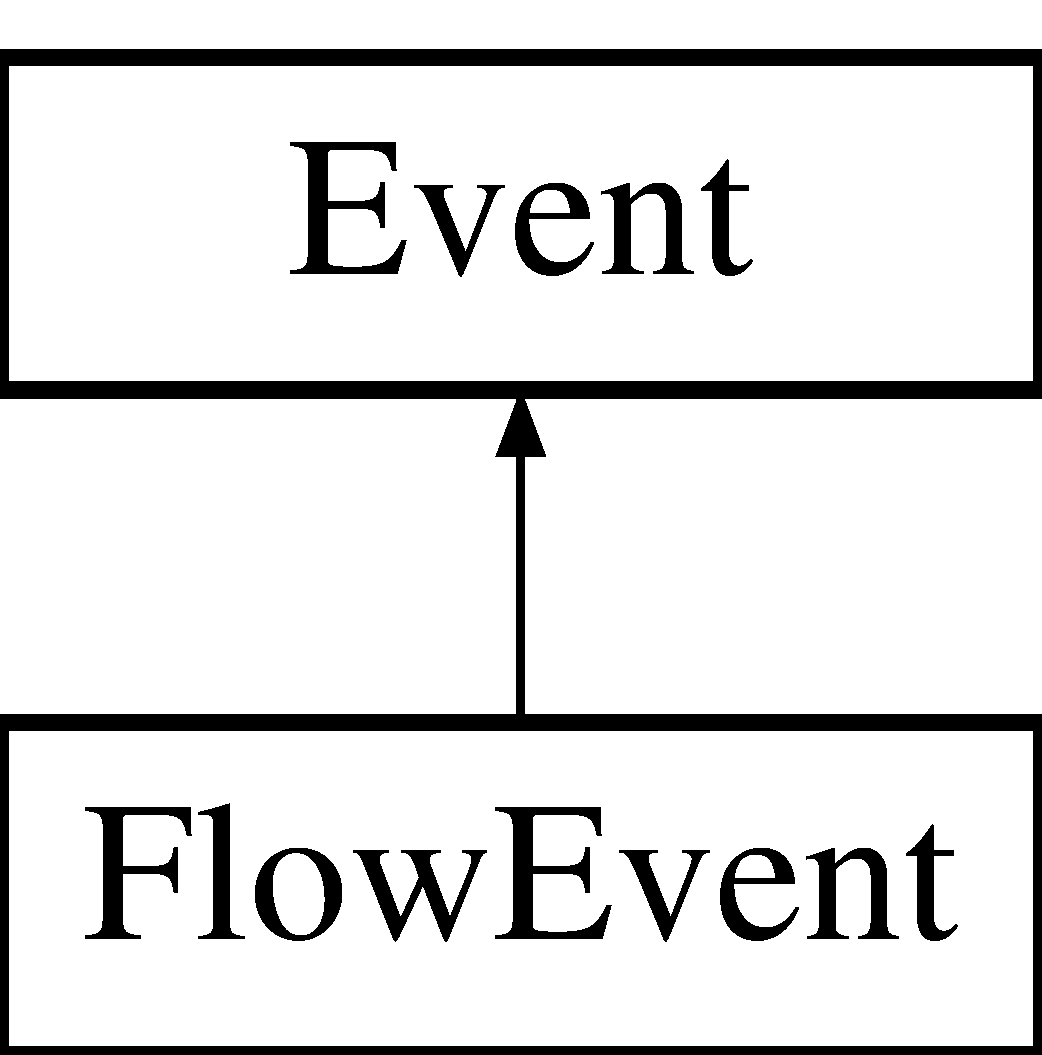
\includegraphics[height=2.000000cm]{classFlowEvent}
\end{center}
\end{figure}
\subsection*{\-Public \-Member \-Functions}
\begin{DoxyCompactItemize}
\item 
\hypertarget{classFlowEvent_a847531a58e1e8ff6adf4a51fad9cc2c0}{{\bfseries \-Flow\-Event} (std\-::shared\-\_\-ptr$<$ \hyperlink{classFlow}{\-Flow} $>$ flowobj, std\-::string dest, std\-::string src, float ts)}\label{classFlowEvent_a847531a58e1e8ff6adf4a51fad9cc2c0}

\item 
\hypertarget{classFlowEvent_a96fc31ece4164d62db961a1ae6862e70}{virtual std\-::string {\bfseries print\-Event} () override}\label{classFlowEvent_a96fc31ece4164d62db961a1ae6862e70}

\item 
\hypertarget{classFlowEvent_a6712fde91ba4bbe86918315e85dff998}{virtual std\-::string {\bfseries get\-Type} () override}\label{classFlowEvent_a6712fde91ba4bbe86918315e85dff998}

\end{DoxyCompactItemize}
\subsection*{\-Public \-Attributes}
\begin{DoxyCompactItemize}
\item 
\hypertarget{classFlowEvent_ae6010e994bd60eff8cb63478f1df0f40}{int {\bfseries data\-\_\-size}}\label{classFlowEvent_ae6010e994bd60eff8cb63478f1df0f40}

\item 
\hypertarget{classFlowEvent_ad0ecfc4035bbfcfaa16f87fcea1b90f2}{std\-::shared\-\_\-ptr$<$ \hyperlink{classFlow}{\-Flow} $>$ {\bfseries floww}}\label{classFlowEvent_ad0ecfc4035bbfcfaa16f87fcea1b90f2}

\end{DoxyCompactItemize}


\-The documentation for this class was generated from the following files\-:\begin{DoxyCompactItemize}
\item 
\-Flow\-Event.\-h\item 
\-Flow\-Event.\-cpp\end{DoxyCompactItemize}

\hypertarget{classFlowGenerator}{\section{\-Flow\-Generator \-Class \-Reference}
\label{classFlowGenerator}\index{\-Flow\-Generator@{\-Flow\-Generator}}
}


\-An object used to store \hyperlink{classFlow}{\-Flow} objects until the data flow is ready to begin.  




{\ttfamily \#include $<$\-Flow\-Generator.\-h$>$}

\-Inheritance diagram for \-Flow\-Generator\-:\begin{figure}[H]
\begin{center}
\leavevmode
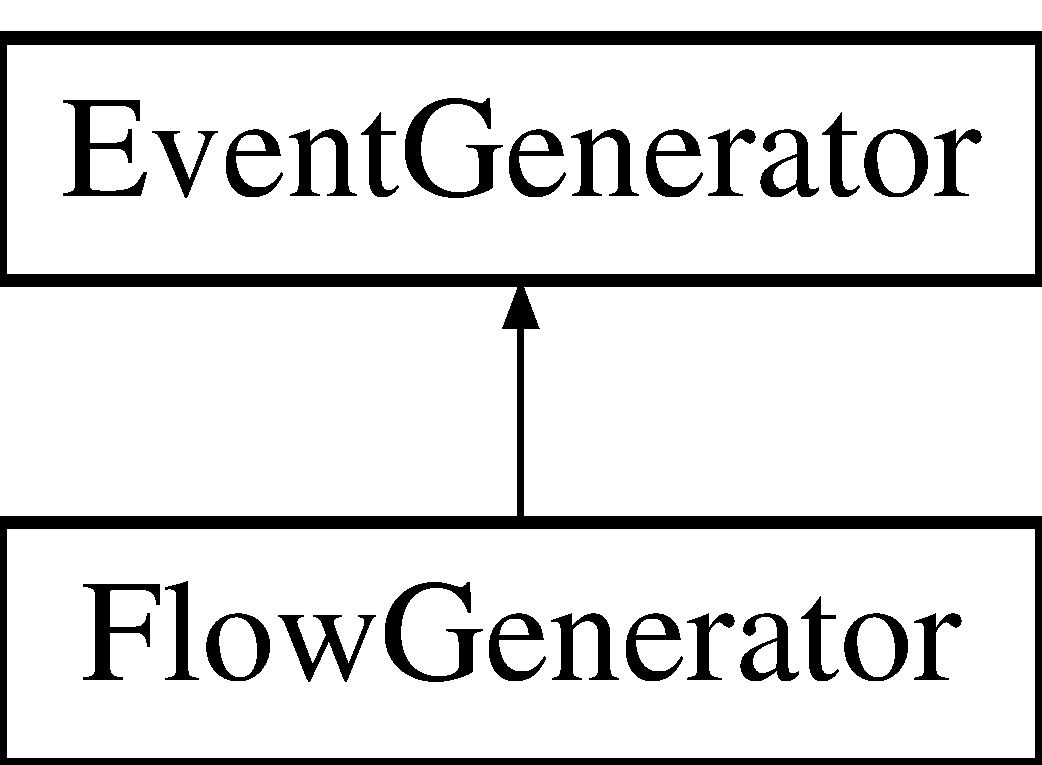
\includegraphics[height=2.000000cm]{classFlowGenerator}
\end{center}
\end{figure}
\subsection*{\-Public \-Member \-Functions}
\begin{DoxyCompactItemize}
\item 
\hyperlink{classFlowGenerator_ae51c2e304770a911f9cc1d8e0d01310c}{\-Flow\-Generator} (std\-::vector$<$ std\-::shared\-\_\-ptr$<$ \hyperlink{classFlow}{\-Flow} $>$ $>$ flows, std\-::string flow\-\_\-id)
\begin{DoxyCompactList}\small\item\em \-Creates a \hyperlink{classFlowGenerator}{\-Flow\-Generator} object. \end{DoxyCompactList}\item 
void \hyperlink{classFlowGenerator_a9fd8f79663c4af4ab229dde250bc258c}{give\-Event} (std\-::shared\-\_\-ptr$<$ \hyperlink{classEvent}{\-Event} $>$ e)
\begin{DoxyCompactList}\small\item\em \-This method should never be called on the \hyperlink{classFlowGenerator}{\-Flow\-Generator}, since it cannot receive events. \end{DoxyCompactList}\end{DoxyCompactItemize}


\subsection{\-Detailed \-Description}
\-An object used to store \hyperlink{classFlow}{\-Flow} objects until the data flow is ready to begin. 

\-It holds an event\-\_\-heap of \-Flow\-Events that are passed to the \hyperlink{classHandler}{\-Handler} when the data flow should begin. \-The \hyperlink{classHandler}{\-Handler} processes these \-Flow\-Events, and creates a data flow on the proper \hyperlink{classHost}{\-Host}. 

\subsection{\-Constructor \& \-Destructor \-Documentation}
\hypertarget{classFlowGenerator_ae51c2e304770a911f9cc1d8e0d01310c}{\index{\-Flow\-Generator@{\-Flow\-Generator}!\-Flow\-Generator@{\-Flow\-Generator}}
\index{\-Flow\-Generator@{\-Flow\-Generator}!FlowGenerator@{\-Flow\-Generator}}
\subsubsection[{\-Flow\-Generator}]{\setlength{\rightskip}{0pt plus 5cm}{\bf \-Flow\-Generator\-::\-Flow\-Generator} (
\begin{DoxyParamCaption}
\item[{std\-::vector$<$ std\-::shared\-\_\-ptr$<$ {\bf \-Flow} $>$ $>$}]{flows, }
\item[{std\-::string}]{flow\-\_\-id}
\end{DoxyParamCaption}
)}}\label{classFlowGenerator_ae51c2e304770a911f9cc1d8e0d01310c}


\-Creates a \hyperlink{classFlowGenerator}{\-Flow\-Generator} object. 

\-The constructor takes in a list of flows, which is uses to populate its event\-\_\-heap with \-Flow\-Events. \-These events are fired at the appropriate times by the \hyperlink{classHandler}{\-Handler} to start the data flows.


\begin{DoxyParams}{\-Parameters}
{\em flows} & the list of flows. \\
\hline
{\em flow\-\_\-id} & the id of the flow generator. \\
\hline
\end{DoxyParams}


\subsection{\-Member \-Function \-Documentation}
\hypertarget{classFlowGenerator_a9fd8f79663c4af4ab229dde250bc258c}{\index{\-Flow\-Generator@{\-Flow\-Generator}!give\-Event@{give\-Event}}
\index{give\-Event@{give\-Event}!FlowGenerator@{\-Flow\-Generator}}
\subsubsection[{give\-Event}]{\setlength{\rightskip}{0pt plus 5cm}void {\bf \-Flow\-Generator\-::give\-Event} (
\begin{DoxyParamCaption}
\item[{std\-::shared\-\_\-ptr$<$ {\bf \-Event} $>$}]{e}
\end{DoxyParamCaption}
)\hspace{0.3cm}{\ttfamily  \mbox{[}virtual\mbox{]}}}}\label{classFlowGenerator_a9fd8f79663c4af4ab229dde250bc258c}


\-This method should never be called on the \hyperlink{classFlowGenerator}{\-Flow\-Generator}, since it cannot receive events. 


\begin{DoxyParams}{\-Parameters}
{\em e} & the event given to the \hyperlink{classFlowGenerator}{\-Flow\-Generator}. \\
\hline
\end{DoxyParams}


\-Implements \hyperlink{classEventGenerator_a7448c87e533a9b38c20d914fa6a13c8e}{\-Event\-Generator}.



\-The documentation for this class was generated from the following files\-:\begin{DoxyCompactItemize}
\item 
/home/max/caltech/\-Net\-Sim/\-C\-S\-\_\-143/src/\-Event\-Generators/\-Flow\-Generator.\-h\item 
/home/max/caltech/\-Net\-Sim/\-C\-S\-\_\-143/src/\-Event\-Generators/\-Flow\-Generator.\-cpp\end{DoxyCompactItemize}

\hypertarget{classHandler}{\section{\-Handler \-Class \-Reference}
\label{classHandler}\index{\-Handler@{\-Handler}}
}
\subsection*{\-Public \-Member \-Functions}
\begin{DoxyCompactItemize}
\item 
\hypertarget{classHandler_aeb01be730be52d6ef994656d40a006ee}{float {\bfseries get\-Min\-Time} ()}\label{classHandler_aeb01be730be52d6ef994656d40a006ee}

\item 
\hypertarget{classHandler_ad81950f9fe02ec3c50f65ee3eb251738}{void {\bfseries populate\-Current\-Events} (float time)}\label{classHandler_ad81950f9fe02ec3c50f65ee3eb251738}

\item 
\hypertarget{classHandler_ad67c5bf3357aba8c6b71fa76c5161d29}{void {\bfseries process\-Current\-Events} ()}\label{classHandler_ad67c5bf3357aba8c6b71fa76c5161d29}

\item 
\hypertarget{classHandler_aa60626b419730f48a1bd5b91c9ade9d7}{void {\bfseries step} ()}\label{classHandler_aa60626b419730f48a1bd5b91c9ade9d7}

\item 
\hypertarget{classHandler_a6d66a0dfe17658e9ba92080d506654ac}{void {\bfseries add\-Generator} (std\-::shared\-\_\-ptr$<$ \hyperlink{classEventGenerator}{\-Event\-Generator} $>$ gen)}\label{classHandler_a6d66a0dfe17658e9ba92080d506654ac}

\item 
\hypertarget{classHandler_a1f9bd53a9251f712c6ff20ca48122e6f}{void {\bfseries handle\-Event} (std\-::shared\-\_\-ptr$<$ \hyperlink{classEvent}{\-Event} $>$ event)}\label{classHandler_a1f9bd53a9251f712c6ff20ca48122e6f}

\item 
\hypertarget{classHandler_a4639718d2f590ebd22d0d949a239327d}{bool {\bfseries running} ()}\label{classHandler_a4639718d2f590ebd22d0d949a239327d}

\end{DoxyCompactItemize}


\-The documentation for this class was generated from the following files\-:\begin{DoxyCompactItemize}
\item 
\-Handler.\-h\item 
\-Handler.\-cpp\end{DoxyCompactItemize}

\hypertarget{classHost}{\section{\-Host \-Class \-Reference}
\label{classHost}\index{\-Host@{\-Host}}
}
\-Inheritance diagram for \-Host\-:\begin{figure}[H]
\begin{center}
\leavevmode
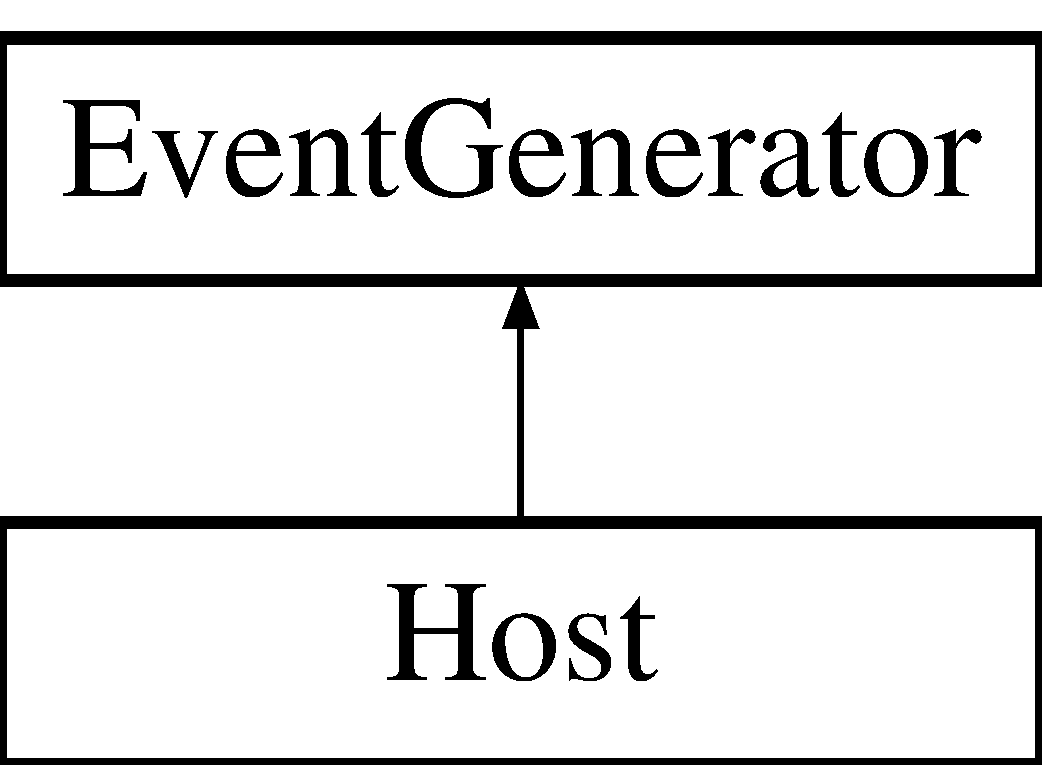
\includegraphics[height=2.000000cm]{classHost}
\end{center}
\end{figure}
\subsection*{\-Public \-Member \-Functions}
\begin{DoxyCompactItemize}
\item 
\hypertarget{classHost_afde96dd6239594d91697006a850bea5b}{{\bfseries \-Host} (std\-::shared\-\_\-ptr$<$ \hyperlink{classLink}{\-Link} $>$ host\-\_\-link, std\-::string host\-\_\-id)}\label{classHost_afde96dd6239594d91697006a850bea5b}

\item 
\hypertarget{classHost_a658a8bee30dfb9e6ff7abc26620f88ff}{virtual void {\bfseries give\-Event} (std\-::shared\-\_\-ptr$<$ \hyperlink{classEvent}{\-Event} $>$) override}\label{classHost_a658a8bee30dfb9e6ff7abc26620f88ff}

\item 
void \hyperlink{classHost_a28da4a1168cd8ce7c396f0ba5ced1c66}{respond\-To} (\hyperlink{classPacketEvent}{\-Packet\-Event})
\item 
\hypertarget{classHost_adbd4abe19840d56b09499af1158d6081}{void {\bfseries respond\-To} (\hyperlink{classFlowEvent}{\-Flow\-Event})}\label{classHost_adbd4abe19840d56b09499af1158d6081}

\item 
void \hyperlink{classHost_a64221eb13d89a1bb84f1eb351bc45be4}{respond\-To} (\hyperlink{classUnackEvent}{\-Unack\-Event})
\item 
\hypertarget{classHost_aa807c50f690bd2018265504483440c7d}{std\-::string {\bfseries to\-String} ()}\label{classHost_aa807c50f690bd2018265504483440c7d}

\end{DoxyCompactItemize}
\subsection*{\-Public \-Attributes}
\begin{DoxyCompactItemize}
\item 
\hypertarget{classHost_a6b880d3ae2688e05f0617de4c247b84c}{std\-::shared\-\_\-ptr$<$ \hyperlink{classLink}{\-Link} $>$ {\bfseries my\-\_\-link}}\label{classHost_a6b880d3ae2688e05f0617de4c247b84c}

\item 
\hypertarget{classHost_a27e0ce48916f5882e8916f96ec1a6b1f}{std\-::unordered\-\_\-map\*
$<$ std\-::string, std\-::shared\-\_\-ptr\*
$<$ \hyperlink{classFlow}{\-Flow} $>$ $>$ {\bfseries flows}}\label{classHost_a27e0ce48916f5882e8916f96ec1a6b1f}

\end{DoxyCompactItemize}


\subsection{\-Member \-Function \-Documentation}
\hypertarget{classHost_a28da4a1168cd8ce7c396f0ba5ced1c66}{\index{\-Host@{\-Host}!respond\-To@{respond\-To}}
\index{respond\-To@{respond\-To}!Host@{\-Host}}
\subsubsection[{respond\-To}]{\setlength{\rightskip}{0pt plus 5cm}void {\bf \-Host\-::respond\-To} (
\begin{DoxyParamCaption}
\item[{{\bf \-Packet\-Event}}]{new\-\_\-event}
\end{DoxyParamCaption}
)}}\label{classHost_a28da4a1168cd8ce7c396f0ba5ced1c66}
\-Called when host receives any packet. \hypertarget{classHost_a64221eb13d89a1bb84f1eb351bc45be4}{\index{\-Host@{\-Host}!respond\-To@{respond\-To}}
\index{respond\-To@{respond\-To}!Host@{\-Host}}
\subsubsection[{respond\-To}]{\setlength{\rightskip}{0pt plus 5cm}void {\bf \-Host\-::respond\-To} (
\begin{DoxyParamCaption}
\item[{{\bf \-Unack\-Event}}]{unack\-\_\-event}
\end{DoxyParamCaption}
)}}\label{classHost_a64221eb13d89a1bb84f1eb351bc45be4}
\-Called when there is a potentially unacknowledged packet. 

\-The documentation for this class was generated from the following files\-:\begin{DoxyCompactItemize}
\item 
/home/max/caltech/senior/\-Net\-Sim/\-C\-S\-\_\-143/src/\-Event\-Generators/\-Host.\-h\item 
/home/max/caltech/senior/\-Net\-Sim/\-C\-S\-\_\-143/src/\-Event\-Generators/\-Host.\-cpp\end{DoxyCompactItemize}

\hypertarget{classLink}{\section{\-Link \-Class \-Reference}
\label{classLink}\index{\-Link@{\-Link}}
}


\-Implementation of \-Network \-Links.  




{\ttfamily \#include $<$\-Link.\-h$>$}

\-Inheritance diagram for \-Link\-:\begin{figure}[H]
\begin{center}
\leavevmode
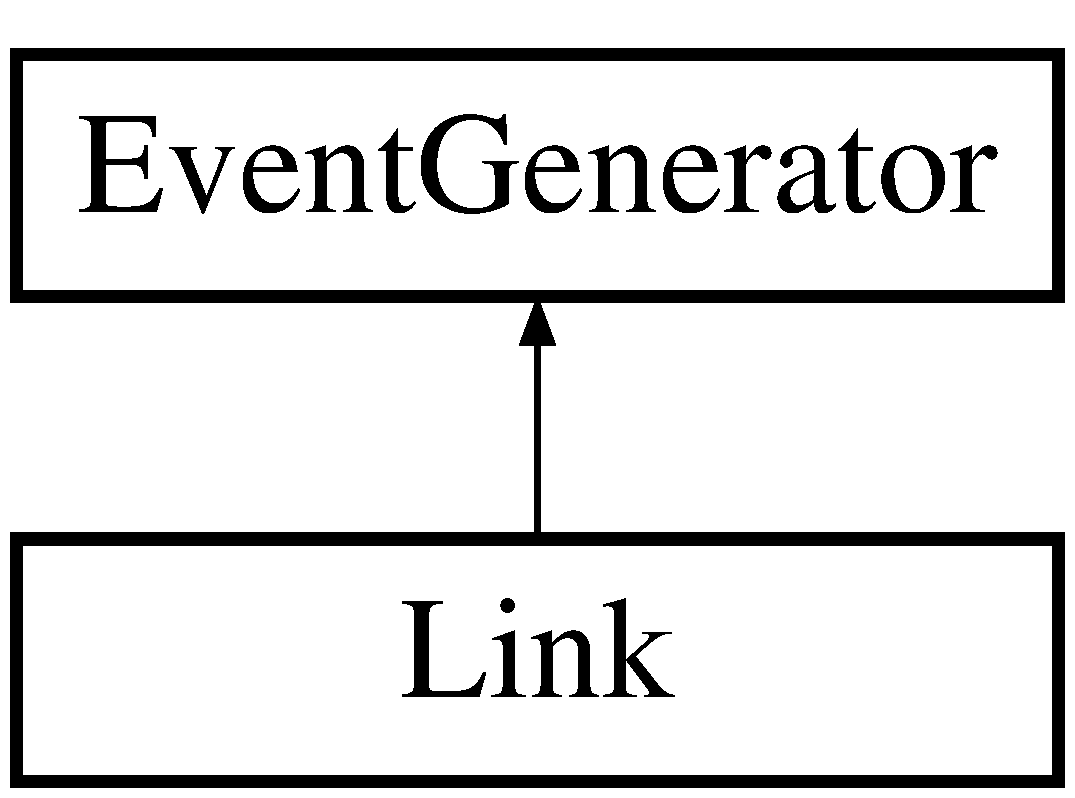
\includegraphics[height=2.000000cm]{classLink}
\end{center}
\end{figure}
\subsection*{\-Public \-Member \-Functions}
\begin{DoxyCompactItemize}
\item 
\hyperlink{classLink_af0a6ae4d9767bacfb371f52a30441e64}{\-Link} (double, float, float, std\-::string, std\-::string, std\-::string)
\begin{DoxyCompactList}\small\item\em \-Constructor for \hyperlink{classLink}{\-Link}. \end{DoxyCompactList}\item 
double \hyperlink{classLink_a19a132f87f8028ccd5af2503084aac64}{get\-Total\-Delay} (std\-::string node)
\begin{DoxyCompactList}\small\item\em \-Gets the total delay of the link seen by a given sending node. \end{DoxyCompactList}\item 
\hypertarget{classLink_a94f034f0b3ebfbf4c08bcae80a5d9904}{void {\bfseries packet\-Loss} (double)}\label{classLink_a94f034f0b3ebfbf4c08bcae80a5d9904}

\item 
double \hyperlink{classLink_a6349999e40910091ecea77e2a366aa46}{get\-Prop\-Delay} ()
\begin{DoxyCompactList}\small\item\em \-Gets the propagation delay of a link. \end{DoxyCompactList}\item 
std\-::string \hyperlink{classLink_a8c768141c7ebf3b852bf978757f903be}{to\-String} ()
\begin{DoxyCompactList}\small\item\em \-Represents the link as a string. \end{DoxyCompactList}\item 
virtual void \hyperlink{classLink_abd9466c4c2097329f4affd9b2eafbd7a}{give\-Event} (std\-::shared\-\_\-ptr$<$ \hyperlink{classEvent}{\-Event} $>$) override
\begin{DoxyCompactList}\small\item\em \-Give the link an event. \end{DoxyCompactList}\item 
std\-::string \hyperlink{classLink_aaa4e4c72a6384f118846765c296e5634}{get\-Other\-Node} (std\-::string node)
\begin{DoxyCompactList}\small\item\em \-Gets the other node connected to a link. \end{DoxyCompactList}\item 
void \hyperlink{classLink_a0e1ec62377102139e4acc14392e96c12}{log\-Link\-Rate} (double time, std\-::string node)
\begin{DoxyCompactList}\small\item\em \-Logs the link rate at a given time for a given sending node. \end{DoxyCompactList}\item 
void \hyperlink{classLink_af07994bcf90cd63abe9edab218a5d752}{log\-Buffer\-Occupancy} (double time, std\-::string node)
\begin{DoxyCompactList}\small\item\em \-Logs the buffer occupancy at a given time for a given sending node. \end{DoxyCompactList}\end{DoxyCompactItemize}


\subsection{\-Detailed \-Description}
\-Implementation of \-Network \-Links. 

\-Links are bi-\/directional, and contain two send buffers. 

\subsection{\-Constructor \& \-Destructor \-Documentation}
\hypertarget{classLink_af0a6ae4d9767bacfb371f52a30441e64}{\index{\-Link@{\-Link}!\-Link@{\-Link}}
\index{\-Link@{\-Link}!Link@{\-Link}}
\subsubsection[{\-Link}]{\setlength{\rightskip}{0pt plus 5cm}{\bf \-Link\-::\-Link} (
\begin{DoxyParamCaption}
\item[{double}]{buf\-\_\-size, }
\item[{float}]{p\-\_\-delay, }
\item[{float}]{cap, }
\item[{std\-::string}]{n1, }
\item[{std\-::string}]{n2, }
\item[{std\-::string}]{link\-\_\-id}
\end{DoxyParamCaption}
)}}\label{classLink_af0a6ae4d9767bacfb371f52a30441e64}


\-Constructor for \hyperlink{classLink}{\-Link}. 


\begin{DoxyParams}{\-Parameters}
{\em buf\-\_\-size} & the size of the link buffers. \\
\hline
{\em p\-\_\-delay} & the propagation delay of the link. \\
\hline
{\em cap} & the link capacity. \\
\hline
{\em n1} & a device connected to the link. \\
\hline
{\em n2} & a device connected to the link. \\
\hline
{\em link\-\_\-id} & the name of the link. \\
\hline
\end{DoxyParams}


\subsection{\-Member \-Function \-Documentation}
\hypertarget{classLink_aaa4e4c72a6384f118846765c296e5634}{\index{\-Link@{\-Link}!get\-Other\-Node@{get\-Other\-Node}}
\index{get\-Other\-Node@{get\-Other\-Node}!Link@{\-Link}}
\subsubsection[{get\-Other\-Node}]{\setlength{\rightskip}{0pt plus 5cm}std\-::string {\bf \-Link\-::get\-Other\-Node} (
\begin{DoxyParamCaption}
\item[{std\-::string}]{my\-\_\-node}
\end{DoxyParamCaption}
)}}\label{classLink_aaa4e4c72a6384f118846765c296e5634}


\-Gets the other node connected to a link. 


\begin{DoxyParams}{\-Parameters}
{\em node} & the node we know about. \\
\hline
\end{DoxyParams}
\begin{DoxyReturn}{\-Returns}
the node on the opposite end. 
\end{DoxyReturn}
\hypertarget{classLink_a6349999e40910091ecea77e2a366aa46}{\index{\-Link@{\-Link}!get\-Prop\-Delay@{get\-Prop\-Delay}}
\index{get\-Prop\-Delay@{get\-Prop\-Delay}!Link@{\-Link}}
\subsubsection[{get\-Prop\-Delay}]{\setlength{\rightskip}{0pt plus 5cm}double {\bf \-Link\-::get\-Prop\-Delay} (
\begin{DoxyParamCaption}
{}
\end{DoxyParamCaption}
)}}\label{classLink_a6349999e40910091ecea77e2a366aa46}


\-Gets the propagation delay of a link. 

\begin{DoxyReturn}{\-Returns}
the propagation delay of the link. 
\end{DoxyReturn}
\hypertarget{classLink_a19a132f87f8028ccd5af2503084aac64}{\index{\-Link@{\-Link}!get\-Total\-Delay@{get\-Total\-Delay}}
\index{get\-Total\-Delay@{get\-Total\-Delay}!Link@{\-Link}}
\subsubsection[{get\-Total\-Delay}]{\setlength{\rightskip}{0pt plus 5cm}double {\bf \-Link\-::get\-Total\-Delay} (
\begin{DoxyParamCaption}
\item[{std\-::string}]{node}
\end{DoxyParamCaption}
)}}\label{classLink_a19a132f87f8028ccd5af2503084aac64}


\-Gets the total delay of the link seen by a given sending node. 


\begin{DoxyParams}{\-Parameters}
{\em node} & the node seeing the delay. \\
\hline
\end{DoxyParams}
\begin{DoxyReturn}{\-Returns}
total delay 
\end{DoxyReturn}
\hypertarget{classLink_abd9466c4c2097329f4affd9b2eafbd7a}{\index{\-Link@{\-Link}!give\-Event@{give\-Event}}
\index{give\-Event@{give\-Event}!Link@{\-Link}}
\subsubsection[{give\-Event}]{\setlength{\rightskip}{0pt plus 5cm}void {\bf \-Link\-::give\-Event} (
\begin{DoxyParamCaption}
\item[{std\-::shared\-\_\-ptr$<$ {\bf \-Event} $>$}]{e}
\end{DoxyParamCaption}
)\hspace{0.3cm}{\ttfamily  \mbox{[}override, virtual\mbox{]}}}}\label{classLink_abd9466c4c2097329f4affd9b2eafbd7a}


\-Give the link an event. 

\-This method assumes that it is a packet event. \-The link responds by determining whether the packet is dropped or not. \-If the packet is not dropped, it is placed onto the queue for transmission.


\begin{DoxyParams}{\-Parameters}
{\em e} & the packet event given to the link. \\
\hline
\end{DoxyParams}


\-Implements \hyperlink{classEventGenerator_a7448c87e533a9b38c20d914fa6a13c8e}{\-Event\-Generator}.

\hypertarget{classLink_af07994bcf90cd63abe9edab218a5d752}{\index{\-Link@{\-Link}!log\-Buffer\-Occupancy@{log\-Buffer\-Occupancy}}
\index{log\-Buffer\-Occupancy@{log\-Buffer\-Occupancy}!Link@{\-Link}}
\subsubsection[{log\-Buffer\-Occupancy}]{\setlength{\rightskip}{0pt plus 5cm}void {\bf \-Link\-::log\-Buffer\-Occupancy} (
\begin{DoxyParamCaption}
\item[{double}]{time, }
\item[{std\-::string}]{node}
\end{DoxyParamCaption}
)}}\label{classLink_af07994bcf90cd63abe9edab218a5d752}


\-Logs the buffer occupancy at a given time for a given sending node. 


\begin{DoxyParams}{\-Parameters}
{\em node} & the node sending packets down the link. \\
\hline
\end{DoxyParams}
\hypertarget{classLink_a0e1ec62377102139e4acc14392e96c12}{\index{\-Link@{\-Link}!log\-Link\-Rate@{log\-Link\-Rate}}
\index{log\-Link\-Rate@{log\-Link\-Rate}!Link@{\-Link}}
\subsubsection[{log\-Link\-Rate}]{\setlength{\rightskip}{0pt plus 5cm}void {\bf \-Link\-::log\-Link\-Rate} (
\begin{DoxyParamCaption}
\item[{double}]{time, }
\item[{std\-::string}]{node}
\end{DoxyParamCaption}
)}}\label{classLink_a0e1ec62377102139e4acc14392e96c12}


\-Logs the link rate at a given time for a given sending node. 


\begin{DoxyParams}{\-Parameters}
{\em node} & the node sending packets down the link. \\
\hline
\end{DoxyParams}
\hypertarget{classLink_a8c768141c7ebf3b852bf978757f903be}{\index{\-Link@{\-Link}!to\-String@{to\-String}}
\index{to\-String@{to\-String}!Link@{\-Link}}
\subsubsection[{to\-String}]{\setlength{\rightskip}{0pt plus 5cm}std\-::string {\bf \-Link\-::to\-String} (
\begin{DoxyParamCaption}
{}
\end{DoxyParamCaption}
)}}\label{classLink_a8c768141c7ebf3b852bf978757f903be}


\-Represents the link as a string. 

\begin{DoxyReturn}{\-Returns}
the string representing the link. 
\end{DoxyReturn}


\-The documentation for this class was generated from the following files\-:\begin{DoxyCompactItemize}
\item 
/home/max/caltech/\-Net\-Sim/\-C\-S\-\_\-143/src/\-Event\-Generators/\-Link.\-h\item 
/home/max/caltech/\-Net\-Sim/\-C\-S\-\_\-143/src/\-Event\-Generators/\-Link.\-cpp\end{DoxyCompactItemize}

\hypertarget{classPacket}{\section{\-Packet \-Class \-Reference}
\label{classPacket}\index{\-Packet@{\-Packet}}
}
\subsection*{\-Public \-Member \-Functions}
\begin{DoxyCompactItemize}
\item 
\hypertarget{classPacket_adad25df1f7cd92863fe024b611654ca0}{{\bfseries \-Packet} (std\-::string id, std\-::string fd, std\-::string src, int s, bool a, int seq)}\label{classPacket_adad25df1f7cd92863fe024b611654ca0}

\item 
\hypertarget{classPacket_a42b25c5d0ca62985777047ae06c0f299}{{\bfseries \-Packet} (std\-::string id, std\-::string fd, std\-::string src, int s, bool a, int seq, std\-::string flow\-\_\-id)}\label{classPacket_a42b25c5d0ca62985777047ae06c0f299}

\item 
\hypertarget{classPacket_ae8d5dfea51fa7fe55e4705b176f326ec}{{\bfseries \-Packet} (const \hyperlink{classPacket}{\-Packet} \&other)}\label{classPacket_ae8d5dfea51fa7fe55e4705b176f326ec}

\item 
\hypertarget{classPacket_af2fa4ac151c764a022093e7fa826a6c2}{std\-::string {\bfseries print\-Packet} ()}\label{classPacket_af2fa4ac151c764a022093e7fa826a6c2}

\end{DoxyCompactItemize}
\subsection*{\-Public \-Attributes}
\begin{DoxyCompactItemize}
\item 
\hypertarget{classPacket_acaefdb9f910265a1ff97b522a780f088}{std\-::string {\bfseries uuid}}\label{classPacket_acaefdb9f910265a1ff97b522a780f088}

\item 
\hypertarget{classPacket_a14d18bd9829ec1951730bc8bbadb570d}{std\-::string {\bfseries final\-\_\-dest}}\label{classPacket_a14d18bd9829ec1951730bc8bbadb570d}

\item 
\hypertarget{classPacket_a9fdc30310ed4a548f4a51dc6c79442d9}{std\-::string {\bfseries source}}\label{classPacket_a9fdc30310ed4a548f4a51dc6c79442d9}

\item 
\hypertarget{classPacket_ad6c10fc808850949cd3f9b9a2ff018d5}{int {\bfseries size}}\label{classPacket_ad6c10fc808850949cd3f9b9a2ff018d5}

\item 
\hypertarget{classPacket_a1824b08ed28de1f329146d082b6d0dee}{bool {\bfseries ack}}\label{classPacket_a1824b08ed28de1f329146d082b6d0dee}

\item 
\hypertarget{classPacket_ab3bb221061fb274a23f041e4b5e93ce7}{bool {\bfseries bf\-\_\-tbl\-\_\-bit}}\label{classPacket_ab3bb221061fb274a23f041e4b5e93ce7}

\item 
\hypertarget{classPacket_a1dcc152b6caa339c9d6f86c0fcde1c52}{int {\bfseries sequence\-\_\-num}}\label{classPacket_a1dcc152b6caa339c9d6f86c0fcde1c52}

\item 
\hypertarget{classPacket_ad841c025e14798586e5a01dfb17a8e56}{std\-::string {\bfseries flow\-I\-D}}\label{classPacket_ad841c025e14798586e5a01dfb17a8e56}

\end{DoxyCompactItemize}


\-The documentation for this class was generated from the following files\-:\begin{DoxyCompactItemize}
\item 
\-Packet.\-h\item 
\-Packet.\-cpp\end{DoxyCompactItemize}

\hypertarget{classPacketEvent}{\section{\-Packet\-Event \-Class \-Reference}
\label{classPacketEvent}\index{\-Packet\-Event@{\-Packet\-Event}}
}
\-Inheritance diagram for \-Packet\-Event\-:\begin{figure}[H]
\begin{center}
\leavevmode
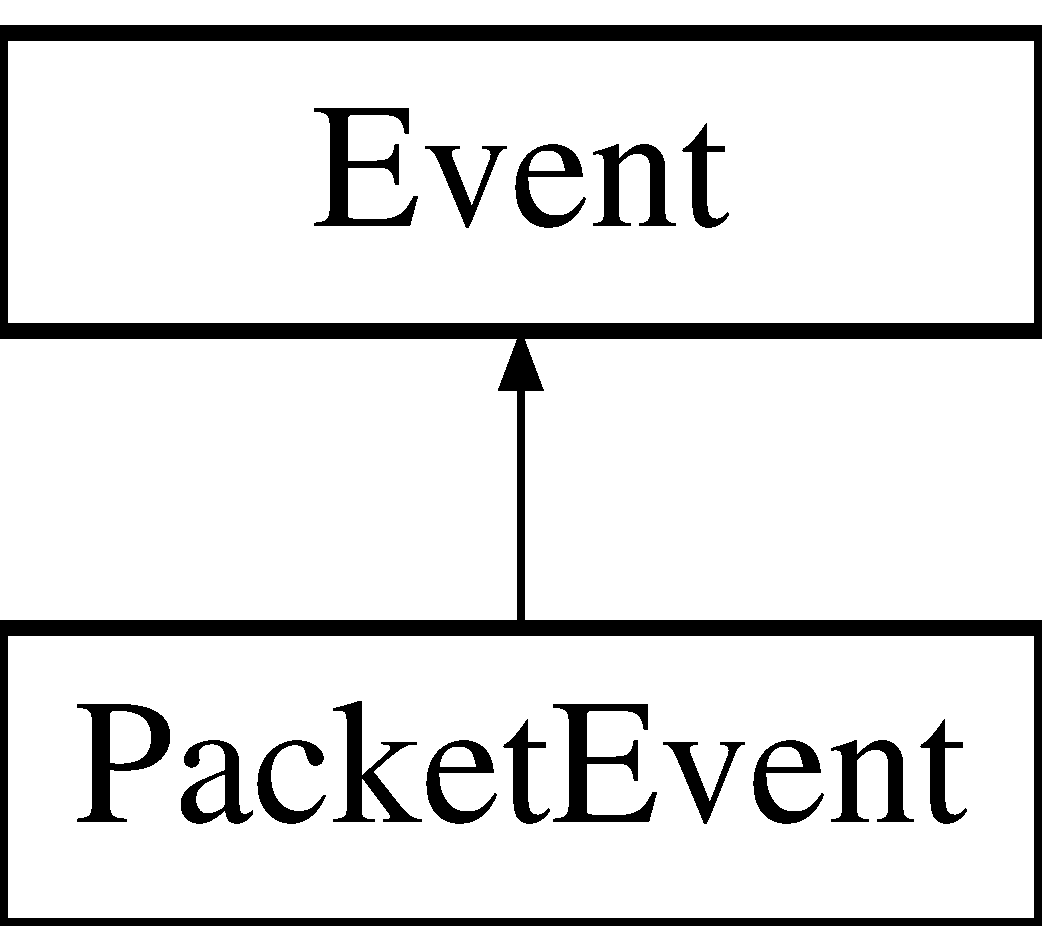
\includegraphics[height=2.000000cm]{classPacketEvent}
\end{center}
\end{figure}
\subsection*{\-Public \-Member \-Functions}
\begin{DoxyCompactItemize}
\item 
\hypertarget{classPacketEvent_a25509c37d21207e1150aa9032eca1a57}{{\bfseries \-Packet\-Event} (std\-::string dest, std\-::string src, float ts, std\-::shared\-\_\-ptr$<$ \hyperlink{classPacket}{\-Packet} $>$ pkt)}\label{classPacketEvent_a25509c37d21207e1150aa9032eca1a57}

\item 
\hypertarget{classPacketEvent_a71221422c26683393ef3a58784f526ff}{virtual std\-::string {\bfseries print\-Event} () override}\label{classPacketEvent_a71221422c26683393ef3a58784f526ff}

\item 
\hypertarget{classPacketEvent_a7dfa4c479200db12df64a12bc39d22d8}{virtual std\-::string {\bfseries get\-Type} () override}\label{classPacketEvent_a7dfa4c479200db12df64a12bc39d22d8}

\end{DoxyCompactItemize}
\subsection*{\-Public \-Attributes}
\begin{DoxyCompactItemize}
\item 
\hypertarget{classPacketEvent_ac3390dfb095c14e0b5c078b51dd914cf}{std\-::shared\-\_\-ptr$<$ \hyperlink{classPacket}{\-Packet} $>$ {\bfseries packet}}\label{classPacketEvent_ac3390dfb095c14e0b5c078b51dd914cf}

\end{DoxyCompactItemize}


\-The documentation for this class was generated from the following files\-:\begin{DoxyCompactItemize}
\item 
\-Packet\-Event.\-h\item 
\-Packet\-Event.\-cpp\end{DoxyCompactItemize}

\input{classPath}
\hypertarget{classRouter}{\section{\-Router \-Class \-Reference}
\label{classRouter}\index{\-Router@{\-Router}}
}
\-Inheritance diagram for \-Router\-:\begin{figure}[H]
\begin{center}
\leavevmode
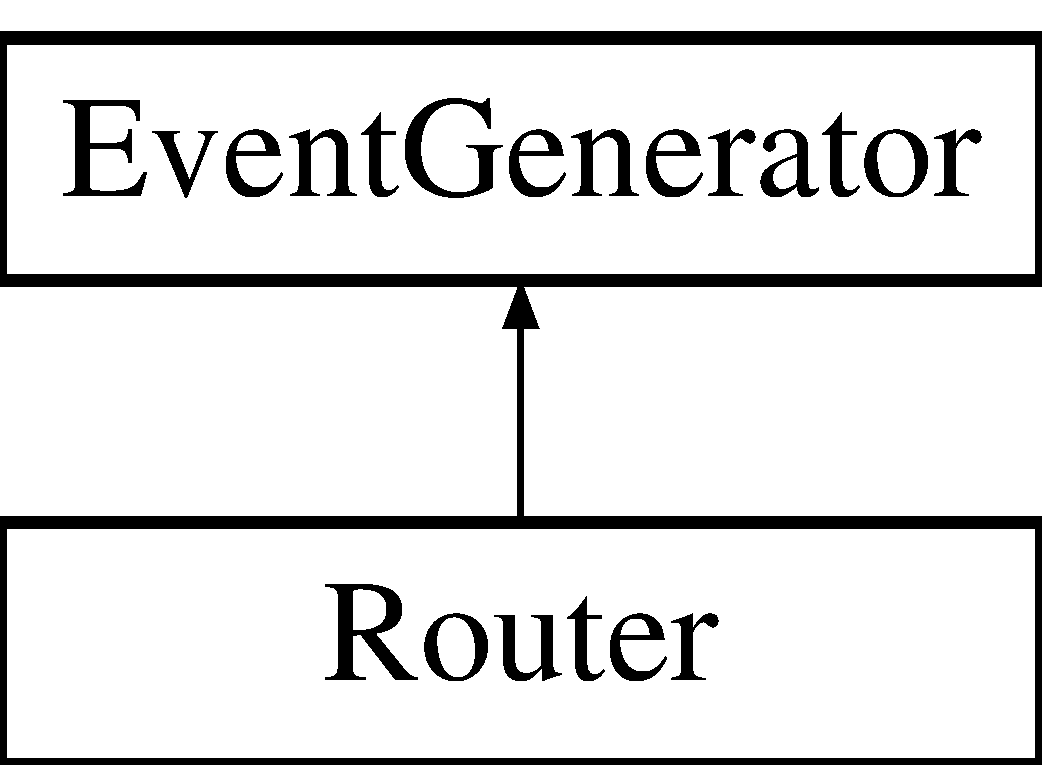
\includegraphics[height=2.000000cm]{classRouter}
\end{center}
\end{figure}
\subsection*{\-Public \-Member \-Functions}
\begin{DoxyCompactItemize}
\item 
\hyperlink{classRouter_a161477ea1b51f59bcd03da20b5d25243}{\-Router} (std\-::vector$<$ std\-::string $>$ host\-\_\-list, std\-::vector$<$ std\-::shared\-\_\-ptr$<$ \hyperlink{classLink}{\-Link} $>$ $>$ neighboring\-\_\-links, std\-::string router\-\_\-id)
\begin{DoxyCompactList}\small\item\em \-Constructor for instance of a \hyperlink{classRouter}{\-Router}. \end{DoxyCompactList}\item 
void \hyperlink{classRouter_a9517660547398a913aab151a3f058fbf}{update\-Routing} (\-Packet\-::bf\-\_\-type, std\-::string, double)
\begin{DoxyCompactList}\small\item\em \-Updates the routing table of a router when it receives a bf\-\_\-packet. \end{DoxyCompactList}\item 
void \hyperlink{classRouter_a0b106e96412284611079588b65721aa6}{broadcast\-Table} (double timestamp)
\begin{DoxyCompactList}\small\item\em \-Broadcasts the routing table to all connected routers. \end{DoxyCompactList}\item 
void \hyperlink{classRouter_a923848a34881212d310a738032d31610}{add\-Routing} (std\-::string targ\-\_\-host, std\-::shared\-\_\-ptr$<$ \hyperlink{classPath}{\-Path} $>$ path)
\begin{DoxyCompactList}\small\item\em \-Adds a host\-\_\-id -\/$>$ (next\-\_\-link\-\_\-id, dist, path) tuple indicating which link to route to given a host, along with bellman-\/ford info. \end{DoxyCompactList}\item 
void \hyperlink{classRouter_aa28dfae66a6e2587d3c39da83059a866}{add\-Link} (std\-::shared\-\_\-ptr$<$ \hyperlink{classLink}{\-Link} $>$ link)
\begin{DoxyCompactList}\small\item\em \-Adds a link to the router's link vector. \end{DoxyCompactList}\item 
std\-::string \hyperlink{classRouter_a2c333b431ae61349b91277cda82a3f5e}{get\-Routing} (std\-::string targ\-\_\-host)
\begin{DoxyCompactList}\small\item\em \-Returns the proper link to route to given a host. \end{DoxyCompactList}\item 
void \hyperlink{classRouter_aed4bdd88f4fa09cb784c5c329c935688}{give\-Event} (std\-::shared\-\_\-ptr$<$ \hyperlink{classEvent}{\-Event} $>$)
\begin{DoxyCompactList}\small\item\em \-Give an event to the router. \end{DoxyCompactList}\item 
\hypertarget{classRouter_aa54f568dd950bcb0feae508e3c75889d}{std\-::string \hyperlink{classRouter_aa54f568dd950bcb0feae508e3c75889d}{to\-String} ()}\label{classRouter_aa54f568dd950bcb0feae508e3c75889d}

\begin{DoxyCompactList}\small\item\em \-Outputs a text representation of a router. \end{DoxyCompactList}\item 
void \hyperlink{classRouter_a323a820ddc17ea36834cf3316510ec5c}{update\-Table\-Weights} (\-Packet\-::bf\-\_\-type)
\begin{DoxyCompactList}\small\item\em \-Updates the link delays in a routing table given a new table. \end{DoxyCompactList}\end{DoxyCompactItemize}


\subsection{\-Constructor \& \-Destructor \-Documentation}
\hypertarget{classRouter_a161477ea1b51f59bcd03da20b5d25243}{\index{\-Router@{\-Router}!\-Router@{\-Router}}
\index{\-Router@{\-Router}!Router@{\-Router}}
\subsubsection[{\-Router}]{\setlength{\rightskip}{0pt plus 5cm}{\bf \-Router\-::\-Router} (
\begin{DoxyParamCaption}
\item[{std\-::vector$<$ std\-::string $>$}]{host\-\_\-list, }
\item[{std\-::vector$<$ std\-::shared\-\_\-ptr$<$ {\bf \-Link} $>$ $>$}]{neighboring\-\_\-links, }
\item[{std\-::string}]{router\-\_\-id}
\end{DoxyParamCaption}
)}}\label{classRouter_a161477ea1b51f59bcd03da20b5d25243}


\-Constructor for instance of a \hyperlink{classRouter}{\-Router}. 


\begin{DoxyParams}{\-Parameters}
{\em host\-\_\-list} & a list of hosts the router connects to. \\
\hline
{\em neighboring\-\_\-links} & a list of pointers to connected links. \\
\hline
{\em router\-\_\-id} & the router name. \\
\hline
\end{DoxyParams}


\subsection{\-Member \-Function \-Documentation}
\hypertarget{classRouter_aa28dfae66a6e2587d3c39da83059a866}{\index{\-Router@{\-Router}!add\-Link@{add\-Link}}
\index{add\-Link@{add\-Link}!Router@{\-Router}}
\subsubsection[{add\-Link}]{\setlength{\rightskip}{0pt plus 5cm}void {\bf \-Router\-::add\-Link} (
\begin{DoxyParamCaption}
\item[{std\-::shared\-\_\-ptr$<$ {\bf \-Link} $>$}]{link}
\end{DoxyParamCaption}
)}}\label{classRouter_aa28dfae66a6e2587d3c39da83059a866}


\-Adds a link to the router's link vector. 


\begin{DoxyParams}{\-Parameters}
{\em link} & a pointer to the link to add. \\
\hline
\end{DoxyParams}
\hypertarget{classRouter_a923848a34881212d310a738032d31610}{\index{\-Router@{\-Router}!add\-Routing@{add\-Routing}}
\index{add\-Routing@{add\-Routing}!Router@{\-Router}}
\subsubsection[{add\-Routing}]{\setlength{\rightskip}{0pt plus 5cm}void {\bf \-Router\-::add\-Routing} (
\begin{DoxyParamCaption}
\item[{std\-::string}]{host\-\_\-id, }
\item[{std\-::shared\-\_\-ptr$<$ {\bf \-Path} $>$}]{path}
\end{DoxyParamCaption}
)}}\label{classRouter_a923848a34881212d310a738032d31610}


\-Adds a host\-\_\-id -\/$>$ (next\-\_\-link\-\_\-id, dist, path) tuple indicating which link to route to given a host, along with bellman-\/ford info. 


\begin{DoxyParams}{\-Parameters}
{\em host\-\_\-id} & the name of the host to which the router is routing packets. \\
\hline
{\em path} & a pointer to the path it will use to route packets. \\
\hline
\end{DoxyParams}
\hypertarget{classRouter_a0b106e96412284611079588b65721aa6}{\index{\-Router@{\-Router}!broadcast\-Table@{broadcast\-Table}}
\index{broadcast\-Table@{broadcast\-Table}!Router@{\-Router}}
\subsubsection[{broadcast\-Table}]{\setlength{\rightskip}{0pt plus 5cm}void {\bf \-Router\-::broadcast\-Table} (
\begin{DoxyParamCaption}
\item[{double}]{timestamp}
\end{DoxyParamCaption}
)}}\label{classRouter_a0b106e96412284611079588b65721aa6}


\-Broadcasts the routing table to all connected routers. 


\begin{DoxyParams}{\-Parameters}
{\em timestamp} & the time at which the broadcast occurs. \\
\hline
\end{DoxyParams}
\hypertarget{classRouter_a2c333b431ae61349b91277cda82a3f5e}{\index{\-Router@{\-Router}!get\-Routing@{get\-Routing}}
\index{get\-Routing@{get\-Routing}!Router@{\-Router}}
\subsubsection[{get\-Routing}]{\setlength{\rightskip}{0pt plus 5cm}std\-::string {\bf \-Router\-::get\-Routing} (
\begin{DoxyParamCaption}
\item[{std\-::string}]{targ\-\_\-host}
\end{DoxyParamCaption}
)}}\label{classRouter_a2c333b431ae61349b91277cda82a3f5e}


\-Returns the proper link to route to given a host. 


\begin{DoxyParams}{\-Parameters}
{\em targ\-\_\-host} & the name of the host to which the router is routing packets. \\
\hline
\end{DoxyParams}
\begin{DoxyReturn}{\-Returns}
the name of the next link in the path. 
\end{DoxyReturn}
\hypertarget{classRouter_aed4bdd88f4fa09cb784c5c329c935688}{\index{\-Router@{\-Router}!give\-Event@{give\-Event}}
\index{give\-Event@{give\-Event}!Router@{\-Router}}
\subsubsection[{give\-Event}]{\setlength{\rightskip}{0pt plus 5cm}void {\bf \-Router\-::give\-Event} (
\begin{DoxyParamCaption}
\item[{std\-::shared\-\_\-ptr$<$ {\bf \-Event} $>$}]{e}
\end{DoxyParamCaption}
)\hspace{0.3cm}{\ttfamily  \mbox{[}virtual\mbox{]}}}}\label{classRouter_aed4bdd88f4fa09cb784c5c329c935688}


\-Give an event to the router. 

\-This method assumes it to be a packet event.


\begin{DoxyParams}{\-Parameters}
{\em e} & the event to be processed \\
\hline
\end{DoxyParams}


\-Implements \hyperlink{classEventGenerator_a7448c87e533a9b38c20d914fa6a13c8e}{\-Event\-Generator}.

\hypertarget{classRouter_a9517660547398a913aab151a3f058fbf}{\index{\-Router@{\-Router}!update\-Routing@{update\-Routing}}
\index{update\-Routing@{update\-Routing}!Router@{\-Router}}
\subsubsection[{update\-Routing}]{\setlength{\rightskip}{0pt plus 5cm}void {\bf \-Router\-::update\-Routing} (
\begin{DoxyParamCaption}
\item[{\-Packet\-::bf\-\_\-type}]{bf\-\_\-table, }
\item[{std\-::string}]{link\-\_\-id, }
\item[{double}]{now}
\end{DoxyParamCaption}
)}}\label{classRouter_a9517660547398a913aab151a3f058fbf}


\-Updates the routing table of a router when it receives a bf\-\_\-packet. 


\begin{DoxyParams}{\-Parameters}
{\em bf\-\_\-table} & the routing table received. \\
\hline
{\em link\-\_\-id} & the name of the link from which the packet was received. \\
\hline
{\em now} & the timestamp of the packet event. \\
\hline
\end{DoxyParams}
\hypertarget{classRouter_a323a820ddc17ea36834cf3316510ec5c}{\index{\-Router@{\-Router}!update\-Table\-Weights@{update\-Table\-Weights}}
\index{update\-Table\-Weights@{update\-Table\-Weights}!Router@{\-Router}}
\subsubsection[{update\-Table\-Weights}]{\setlength{\rightskip}{0pt plus 5cm}void {\bf \-Router\-::update\-Table\-Weights} (
\begin{DoxyParamCaption}
\item[{\-Packet\-::bf\-\_\-type}]{other\-\_\-table}
\end{DoxyParamCaption}
)}}\label{classRouter_a323a820ddc17ea36834cf3316510ec5c}


\-Updates the link delays in a routing table given a new table. 

\-The link delays only change if they see a more current delay in the new table.


\begin{DoxyParams}{\-Parameters}
{\em other\-\_\-table} & the table with new information about link delays \\
\hline
\end{DoxyParams}


\-The documentation for this class was generated from the following files\-:\begin{DoxyCompactItemize}
\item 
/home/max/caltech/\-Net\-Sim/\-C\-S\-\_\-143/src/\-Event\-Generators/\-Router.\-h\item 
/home/max/caltech/\-Net\-Sim/\-C\-S\-\_\-143/src/\-Event\-Generators/\-Router.\-cpp\end{DoxyCompactItemize}

\input{classTahoeFlow}
\input{classTCPVegasUpdateEvent}
\hypertarget{classUnackEvent}{\section{\-Unack\-Event \-Class \-Reference}
\label{classUnackEvent}\index{\-Unack\-Event@{\-Unack\-Event}}
}
\-Inheritance diagram for \-Unack\-Event\-:\begin{figure}[H]
\begin{center}
\leavevmode
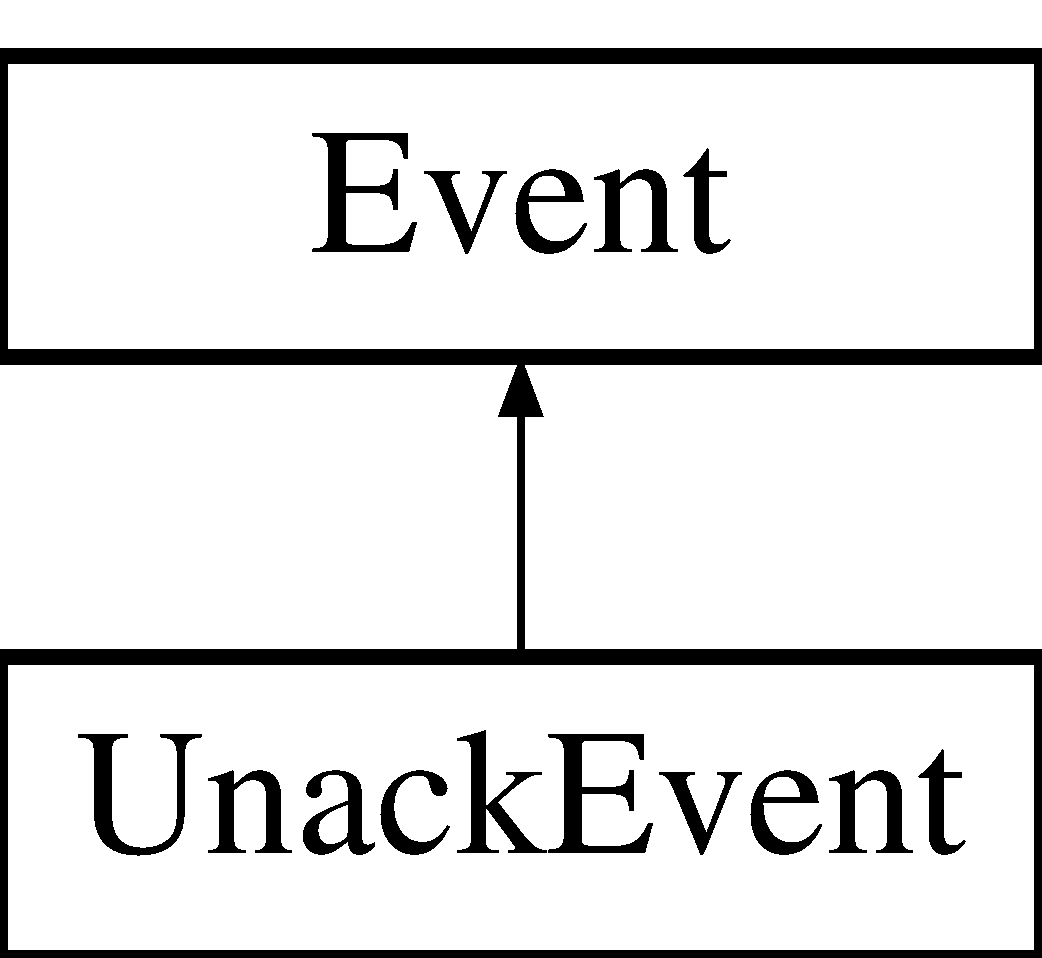
\includegraphics[height=2.000000cm]{classUnackEvent}
\end{center}
\end{figure}
\subsection*{\-Public \-Member \-Functions}
\begin{DoxyCompactItemize}
\item 
\hypertarget{classUnackEvent_abd9be091010bf06561b3b775e914b094}{{\bfseries \-Unack\-Event} (std\-::shared\-\_\-ptr$<$ \hyperlink{classPacket}{\-Packet} $>$ pkt, std\-::string dest, std\-::string src, float ts)}\label{classUnackEvent_abd9be091010bf06561b3b775e914b094}

\item 
\hypertarget{classUnackEvent_a7bc2907c2c7454c761acd654e9b64ca8}{virtual std\-::string {\bfseries print\-Event} () override}\label{classUnackEvent_a7bc2907c2c7454c761acd654e9b64ca8}

\item 
\hypertarget{classUnackEvent_a56ca06731117d1fff95a1601abed02e8}{virtual std\-::string {\bfseries get\-Type} () override}\label{classUnackEvent_a56ca06731117d1fff95a1601abed02e8}

\end{DoxyCompactItemize}
\subsection*{\-Public \-Attributes}
\begin{DoxyCompactItemize}
\item 
\hypertarget{classUnackEvent_ad9d09191d5ee31c15c554e797a708f7d}{std\-::shared\-\_\-ptr$<$ \hyperlink{classPacket}{\-Packet} $>$ {\bfseries packet}}\label{classUnackEvent_ad9d09191d5ee31c15c554e797a708f7d}

\end{DoxyCompactItemize}


\-The documentation for this class was generated from the following files\-:\begin{DoxyCompactItemize}
\item 
\-Unack\-Event.\-h\item 
\-Unack\-Event.\-cpp\end{DoxyCompactItemize}

\input{classVegasFlow}
\printindex
\end{document}
